\documentclass[12pt]{article}
\usepackage{amsmath,amssymb}
\setlength{\oddsidemargin}{0in}
\setlength{\evensidemargin}{0in}
\setlength{\textheight}{9in}
\setlength{\textwidth}{6.5in}
\setlength{\topmargin}{-0.5in}
\usepackage{enumitem}
\usepackage[table]{xcolor}
\usepackage{graphicx}
\usepackage{listings}
\usepackage{float}
\usepackage{caption}
\usepackage{subcaption}

\title{\bf Math 151A: Final}
\date{June 14th, 2023}
\author{\bf Owen Jones}

\begin{document}
\maketitle

\begin{enumerate}[label=\bfseries Problem \arabic*:]
    \item \begin{itemize}
        \item [(a)] $g(x)$ is a continuous function whose derivative $g'(x)=(\sqrt{9-x})'=\frac{-1}{2\sqrt{9-x}}<0$ on the open interal $(0,9)$, in other words decreasing, so $g(x)$ assumes a maximum of $g(0)=3$ at one endpoint and a minimum of $g(9)=0$ at the other. 
        Thus, $g(x)\in[0,9]$ for all $x\in[0,9]$, so $p_k=g(p_{k-1})\in[0,9]$ for all $k\ge0$.
        
        \item [(b)] 
        \begin{align*}
        g(x)\le g(0)=3\text{ if }0\le x\le9\text{ because }g(x)\text{ is a decreasing function.}\\
        \text{Thus, } |g'(g(x))|=|\frac{-1}{2\sqrt{9-\sqrt{9-x}}}|\le|g'(3)|<1\\
        \Rightarrow|g'(p_k)|=|g'(g(p_{k-1}))|\le|g'(3)|<1\text{ for all }k\ge1
        \end{align*}
        Thus, $|g(p_k)-g(p)|\le|g'(3)||p_k-p|\Rightarrow|g(p_k)-g(p)|\le|g'(3)|^2|p_{k-1}-p|\le...\le|g'(3)|^{k-1}|g(p_0)-p|$, so $p_k$ converges to the unique fixed point $p$ for $p_0\in[0,9]$ by the squeeze theorem and the mean value theorem.
        Moreover, $p_k$ converges to the unique fixed point $p$ by a slight variation of the fixed point theorem because $g(p_k)\in[0,9]$ for $p_k\in[0,9]$ and for all but finitely many $|g'(p_k)|$ are bounded above by some $L<1$.
    \end{itemize}
   \newpage
    \item 
    $f(x+h,y)
    =f(x,y)
    +\frac{\partial f(x,y)}{\partial x}h+\frac{\partial f(x,y)}{\partial y}\cdot0
    +\frac{\partial^2 f(x,y)}{\partial x^2}\frac{h^2}{2}+\frac{\partial^2 f(x,y)}{\partial y^2}\cdot0+2\frac{\partial^2 f(x,y)}{\partial x\partial y}\cdot0
    +\frac{\partial^3 f(x,y)}{\partial x^3}\frac{h^3}{6}+3\frac{\partial^3 f(x,y)}{\partial x^2 \partial y}\cdot0+3\frac{\partial^3 f(x,y)}{\partial x\partial y^2}\cdot0+\frac{\partial^3 f(x,y)}{\partial y^3}\cdot0+O(h^4)$\\
    $f(x-h,y)
    =f(x,y)
    +\frac{\partial f(x,y)}{\partial x}(-h)+\frac{\partial f(x,y)}{\partial y}\cdot0
    +\frac{\partial^2 f(x,y)}{\partial x^2}\frac{h^2}{2}+\frac{\partial^2 f(x,y)}{\partial y^2}\cdot0+2\frac{\partial^2 f(x,y)}{\partial x\partial y}\cdot0
    +\frac{\partial^3 f(x,y)}{\partial x^3}\frac{-h^3}{6}+3\frac{\partial^3 f(x,y)}{\partial x^2 \partial y}\cdot0+3\frac{\partial^3 f(x,y)}{\partial x\partial y^2}\cdot0+\frac{\partial^3 f(x,y)}{\partial y^3}\cdot0+O(h^4)$\\
    $f(x,y+h)
    =f(x,y)
    +\frac{\partial f(x,y)}{\partial x}\cdot0+\frac{\partial f(x,y)}{\partial y}h
    +\frac{\partial^2 f(x,y)}{\partial x^2}\cdot0+\frac{\partial^2 f(x,y)}{\partial y^2}\frac{h^2}{2}+2\frac{\partial^2 f(x,y)}{\partial x\partial y}\cdot0
    +\frac{\partial^3 f(x,y)}{\partial x^3}\cdot0+3\frac{\partial^3 f(x,y)}{\partial x^2 \partial y}\cdot0+3\frac{\partial^3 f(x,y)}{\partial x\partial y^2}\cdot0+\frac{\partial^3 f(x,y)}{\partial y^3}\frac{h^3}{6}+O(h^4)$\\
    $f(x,y-h)
    =f(x,y)
    +\frac{\partial f(x,y)}{\partial x}\cdot0+\frac{\partial f(x,y)}{\partial y}(-h)
    +\frac{\partial^2 f(x,y)}{\partial x^2}\cdot0+\frac{\partial^2 f(x,y)}{\partial y^2}\frac{h^2}{2}+2\frac{\partial^2 f(x,y)}{\partial x\partial y}\cdot0
    +\frac{\partial^3 f(x,y)}{\partial x^3}\cdot0+3\frac{\partial^3 f(x,y)}{\partial x^2 \partial y}\cdot0+3\frac{\partial^3 f(x,y)}{\partial x\partial y^2}\cdot0+\frac{\partial^3 f(x,y)}{\partial y^3}\frac{-h^3}{6}+O(h^4)$\\
    $f(x+h,y+h)
    =f(x,y)
    +\frac{\partial f(x,y)}{\partial x}h+\frac{\partial f(x,y)}{\partial y}h
    +\frac{\partial^2 f(x,y)}{\partial x^2}\frac{h^2}{2}+\frac{\partial^2 f(x,y)}{\partial y^2}\frac{h^2}{2}+2\frac{\partial^2 f(x,y)}{\partial x\partial y}\frac{h^2}{2}
    +\frac{\partial^3 f(x,y)}{\partial x^3}\frac{h^3}{6}+3\frac{\partial^3 f(x,y)}{\partial x^2 \partial y}\frac{h^3}{6}+3\frac{\partial^3 f(x,y)}{\partial x\partial y^2}\frac{h^3}{6}+\frac{\partial^3 f(x,y)}{\partial y^3}\frac{h^3}{6}+O(h^4)$\\
    $f(x-h,y-h)
    =f(x,y)
    +\frac{\partial f(x,y)}{\partial x}(-h)+\frac{\partial f(x,y)}{\partial y}(-h)
    +\frac{\partial^2 f(x,y)}{\partial x^2}\frac{h^2}{2}+\frac{\partial^2 f(x,y)}{\partial y^2}\frac{h^2}{2}+2\frac{\partial^2 f(x,y)}{\partial x\partial y}\frac{h^2}{2}
    +\frac{\partial^3 f(x,y)}{\partial x^3}\frac{-h^3}{6}+3\frac{\partial^3 f(x,y)}{\partial x^2 \partial y}\frac{-h^3}{6}+3\frac{\partial^3 f(x,y)}{\partial x\partial y^2}\frac{-h^3}{6}+\frac{\partial^3 f(x,y)}{\partial y^3}\frac{-h^3}{6}+O(h^4)$\\
   
    $\Rightarrow$\\
   
    $0=f(x,y)+\frac{\partial f(x,y)}{\partial x}h+\frac{\partial^2 f(x,y)}{\partial x^2}\frac{h^2}{2}+\frac{\partial^3 f(x,y)}{\partial x^3}\frac{h^3}{6}-f(x+h,y)+O(h^4)$\\
    $0=f(x,y)+\frac{\partial f(x,y)}{\partial x}(-h)+\frac{\partial^2 f(x,y)}{\partial x^2}\frac{h^2}{2}+\frac{\partial^3 f(x,y)}{\partial x^3}\frac{-h^3}{6}-f(x-h,y)+O(h^4)$\\
    $0=f(x,y)+\frac{\partial f(x,y)}{\partial y}h+\frac{\partial^2 f(x,y)}{\partial y^2}\frac{h^2}{2}+\frac{\partial^3 f(x,y)}{\partial y^3}\frac{h^3}{6}-f(x,y+h)+O(h^4)$\\
    $0=f(x,y)+\frac{\partial f(x,y)}{\partial y}(-h)+\frac{\partial^2 f(x,y)}{\partial y^2}\frac{h^2}{2}+\frac{\partial^3 f(x,y)}{\partial y^3}\frac{-h^3}{6}-f(x,y-h)+O(h^4)$\\
    $2\frac{\partial^2 f(x,y)}{\partial x\partial y}\frac{h^2}{2}=-f(x,y)-\frac{\partial f(x,y)}{\partial x}h-\frac{\partial f(x,y)}{\partial y}h-\frac{\partial^2 f(x,y)}{\partial x^2}\frac{h^2}{2}-\frac{\partial^2 f(x,y)}{\partial y^2}\frac{h^2}{2}-\frac{\partial^3 f(x,y)}{\partial x^3}\frac{h^3}{6}-3\frac{\partial^3 f(x,y)}{\partial x^2 \partial y}\frac{h^3}{6}-3\frac{\partial^3 f(x,y)}{\partial x\partial y^2}\frac{h^3}{6}-\frac{\partial^3 f(x,y)}{\partial y^3}\frac{h^3}{6}+f(x+h,y+h)+O(h^4)$\\
    $2\frac{\partial^2 f(x,y)}{\partial x\partial y}\frac{h^2}{2}=-f(x,y)-\frac{\partial f(x,y)}{\partial x}(-h)-\frac{\partial f(x,y)}{\partial y}(-h)-\frac{\partial^2 f(x,y)}{\partial x^2}\frac{h^2}{2}-\frac{\partial^3 f(x,y)}{\partial x^3}\frac{-h^3}{6}-3\frac{\partial^3 f(x,y)}{\partial x^2 \partial y}\frac{-h^3}{6}-3\frac{\partial^3 f(x,y)}{\partial x\partial y^2}\frac{-h^3}{6}-\frac{\partial^3 f(x,y)}{\partial y^3}\frac{-h^3}{6}+f(x-h,y-h)+O(h^4)$\\
   
    $\Rightarrow$\\
   
    $\begin{bmatrix}
    1 & 1 & 1 & 1 & -1 & -1\\
    1 & -1 & 0 & 0 & -1 & 1\\
    0 & 0 & 1 & -1 & -1 & 1\\
    1 & 1 & 0 & 0 & -1 & -1\\
    0 & 0 & 1 & 1 & -1 & -1\\
    0 & 0 & 0 & 0 & -2 & -2
    \end{bmatrix}\cdot
    \begin{bmatrix}
    \frac{1}{2h^2}\\
    \frac{1}{2h^2}\\
    \frac{1}{2h^2}\\
    \frac{1}{2h^2}\\
    \frac{1}{2h^2}\\
    \frac{1}{2h^2} 
    \end{bmatrix}
    =
    \begin{bmatrix}
    \frac{1}{h^2}\\
    0\\
    0\\
    0\\
    0\\
    \frac{-1}{h^2}
    \end{bmatrix}$\\
   
    $\Rightarrow$\\
   
    $\frac{\partial^3 f(x,y)}{\partial x^3}\frac{h^3}{6}\frac{1}{2h^2}+\frac{\partial^3 f(x,y)}{\partial x^3}\frac{-h^3}{6}\frac{1}{2h^2}=0\\
    \frac{\partial^3 f(x,y)}{\partial y^3}\frac{h^3}{6}\frac{1}{2h^2}+\frac{\partial^3 f(x,y)}{\partial y^3}\frac{-h^3}{6}\frac{1}{2h^2}=0\\
    (-\frac{\partial^3 f(x,y)}{\partial x^3}\frac{h^3}{6}-3\frac{\partial^3 f(x,y)}{\partial x^2 \partial y}\frac{h^3}{6}-3\frac{\partial^3 f(x,y)}{\partial x\partial y^2}\frac{h^3}{6}-\frac{\partial^3 f(x,y)}{\partial y^3}\frac{h^3}{6})\frac{1}{2h^2}+(-\frac{\partial^3 f(x,y)}{\partial x^3}\frac{-h^3}{6}-3\frac{\partial^3 f(x,y)}{\partial x^2 \partial y}\frac{-h^3}{6}-3\frac{\partial^3 f(x,y)}{\partial x\partial y^2}\frac{-h^3}{6}-\frac{\partial^3 f(x,y)}{\partial y^3}\frac{-h^3}{6})\frac{1}{2h^2}=0$,\\
    so the $O(h^3)$ terms cancel out by symmetry.\\
    
    $\Rightarrow$\\
    
    $\frac{2\frac{\partial^2 f(x,y)}{\partial x\partial y}\frac{h^2}{2}+2\frac{\partial^2 f(x,y)}{\partial x\partial y}\frac{h^2}{2}}{2h^4}=\frac{h^2(2f(x,y)-f(x+h,y)-f(x-h,y)-f(x,y+h)-f(x,y-h)+f(x+h,y+h)+f(x-h,y-h))+O(h^4)}{2h^4}$\\
    
    $\Rightarrow$\\

    $\frac{\partial^2 f(x,y)}{\partial x\partial y}=\frac{2f(x,y)-f(x+h,y)-f(x-h,y)-f(x,y+h)-f(x,y-h)+f(x+h,y+h)+f(x-h,y-h)}{2h^2}+O(h^2)$\\
    Hence, we obtain the desired result.\\
    \newpage
    \item We have six variables, so we'll need six equations and should expect exactness to at least degree-5.\\
    
    \begin{align*}
        \int_{-1}^{1}1dx=2=c_1\cdot1+c_2\cdot1+c_3\cdot1\\
        \int_{-1}^{1}xdx=0=c_1x_1+x_2x_2+c_3x_3\\
        \int_{-1}^{1}x^2dx=\frac{2}{3}=c_1x^2_1+c_2x^2_2+c_3x^2_3\\
        \int_{-1}^{1}x^3dx=0=c_1x^3_1+c_2x^3_2+c_3x^3_3\\
        \int_{-1}^{1}x^4dx=\frac{2}{5}=c_1x^4_1+c_2x^4_2+c_3x^4_3\\
        \int_{-1}^{1}x^5dx=0=c_1x^5_1+c_2x^5_2+c_3x^5_3\\
    \end{align*}
    Using Wolfram Alpha system of equations solver we obtain
    $\begin{matrix}
        c_1=\frac{5}{9} & c_2=\frac{8}{9} & c_3=\frac{5}{9}\\
        x_1=-\sqrt{\frac{3}{5}} & x_2=0 & x_3=\sqrt{\frac{3}{5}}\\
    \end{matrix}$
    The formula is not exact to degree-6 because $\int_{-1}^{1}x^6dx=\frac{2}{7}\neq c_1x^6_1+c_2x^6_2+c_3x^6_3=\frac{6}{25}$, so our formula is exact to at most degree-5.\\
    \newpage
    \item \begin{itemize}
        \item [(a)] \begin{align*}
        A=\begin{bmatrix}
            10 & -1 & 6\\
            -1 & 8 & 9\\
            6 & 9 & 1\\
        \end{bmatrix}
        \vec{v}^{(0)}=\begin{bmatrix}
            0.5\\
            0.6\\
            0.6\\
        \end{bmatrix}\\
        \vec{w}^{(1)}=A\vec{v}^{(0)}=
        \begin{bmatrix}
            8\\
            \frac{97}{10}\\
            9
        \end{bmatrix}
        ,\vec{v}^{(1)}=\frac{\vec{w}^{(1)}}{||\vec{w}^{(1)}||_2}=
        \begin{bmatrix}
            \frac{80}{\sqrt{23909}}\\
            \frac{97}{\sqrt{23909}}\\
            \frac{90}{\sqrt{23909}}\\
        \end{bmatrix}\\
        \vec{w}^{(2)}=A\vec{v}^{(1)}=
        \begin{bmatrix}
            \frac{1243}{\sqrt{23909}}\\
            \frac{1506}{\sqrt{23909}}\\
            \frac{1443}{\sqrt{23909}}\\
        \end{bmatrix}
        ,\vec{v}^{(2)}=\frac{\vec{w}^{(2)}}{||\vec{w}^{(2)}||_2}=
        \begin{bmatrix}
            \frac{1243}{\sqrt{5895334}}\\
            \frac{753\sqrt{2}}{\sqrt{2947667}}\\
            \frac{1443}{\sqrt{5895334}}\\
        \end{bmatrix}\\
        \lambda^{(2)}=r(\vec{v}^{(2)})=(\vec{v}^{(2)})^TA\vec{v}^{(2)}=\frac{92573743}{5895334}\approx15.7
        \end{align*}
        \item[(b)] \begin{align*}
            \frac{||A\vec{v}^{(2)}-\lambda^{(2)}\vec{v}^{(2)}||_2}{||\lambda^{(2)}\vec{v}^{(2)}||_2}=0.00675
        \end{align*}
        by symbolic solver.
        \item[(c)] \begin{align*}
            \begin{bmatrix}
                10 & -1 & 6\\
                -1 & 8 & 9\\
                6 & 9 & 1\\
            \end{bmatrix}
            -\frac{92573743}{5895334}
            \begin{bmatrix}
                \frac{1243}{\sqrt{5895334}}\\
                \frac{753\sqrt{2}}{\sqrt{2947667}}\\
                \frac{1443}{\sqrt{5895334}}\\
            \end{bmatrix}
            \begin{bmatrix}
                \frac{1243}{\sqrt{5895334}} & \frac{753\sqrt{2}}{\sqrt{2947667}} & \frac{1443}{\sqrt{5895334}}
            \end{bmatrix}\\
            =
            \begin{bmatrix}
                5.88470 & -5.98605 & 1.22255\\
                -5.98605 & 1.95894 & 3.21168\\
                1.22255 & 3.21168 & -4.54613\\
            \end{bmatrix}
        \end{align*}
        \item [(d)] $\vec{v}^{(40)}=\begin{bmatrix}
            0.7982\\
            -0.5990\\
            -0.0639
        \end{bmatrix},
        \lambda^{(40)}=10.2788$ with $tol=10^-5$\\
        $\vec{v}^{(40)}$ and $\lambda^{(40)}$ is an approximation for one of the other two eigenvalue-eigenvector pairs of matrix $A$.\\
        $\frac{A\vec{v}^{(40)}}{\lambda^{(40)}}=\begin{bmatrix}
            0.79752\\
            -0.59980\\
            -0.06476
        \end{bmatrix}$\\
            \begin{figure}[h!]
            \begin{subfigure}{.5\textwidth}
                \centering
               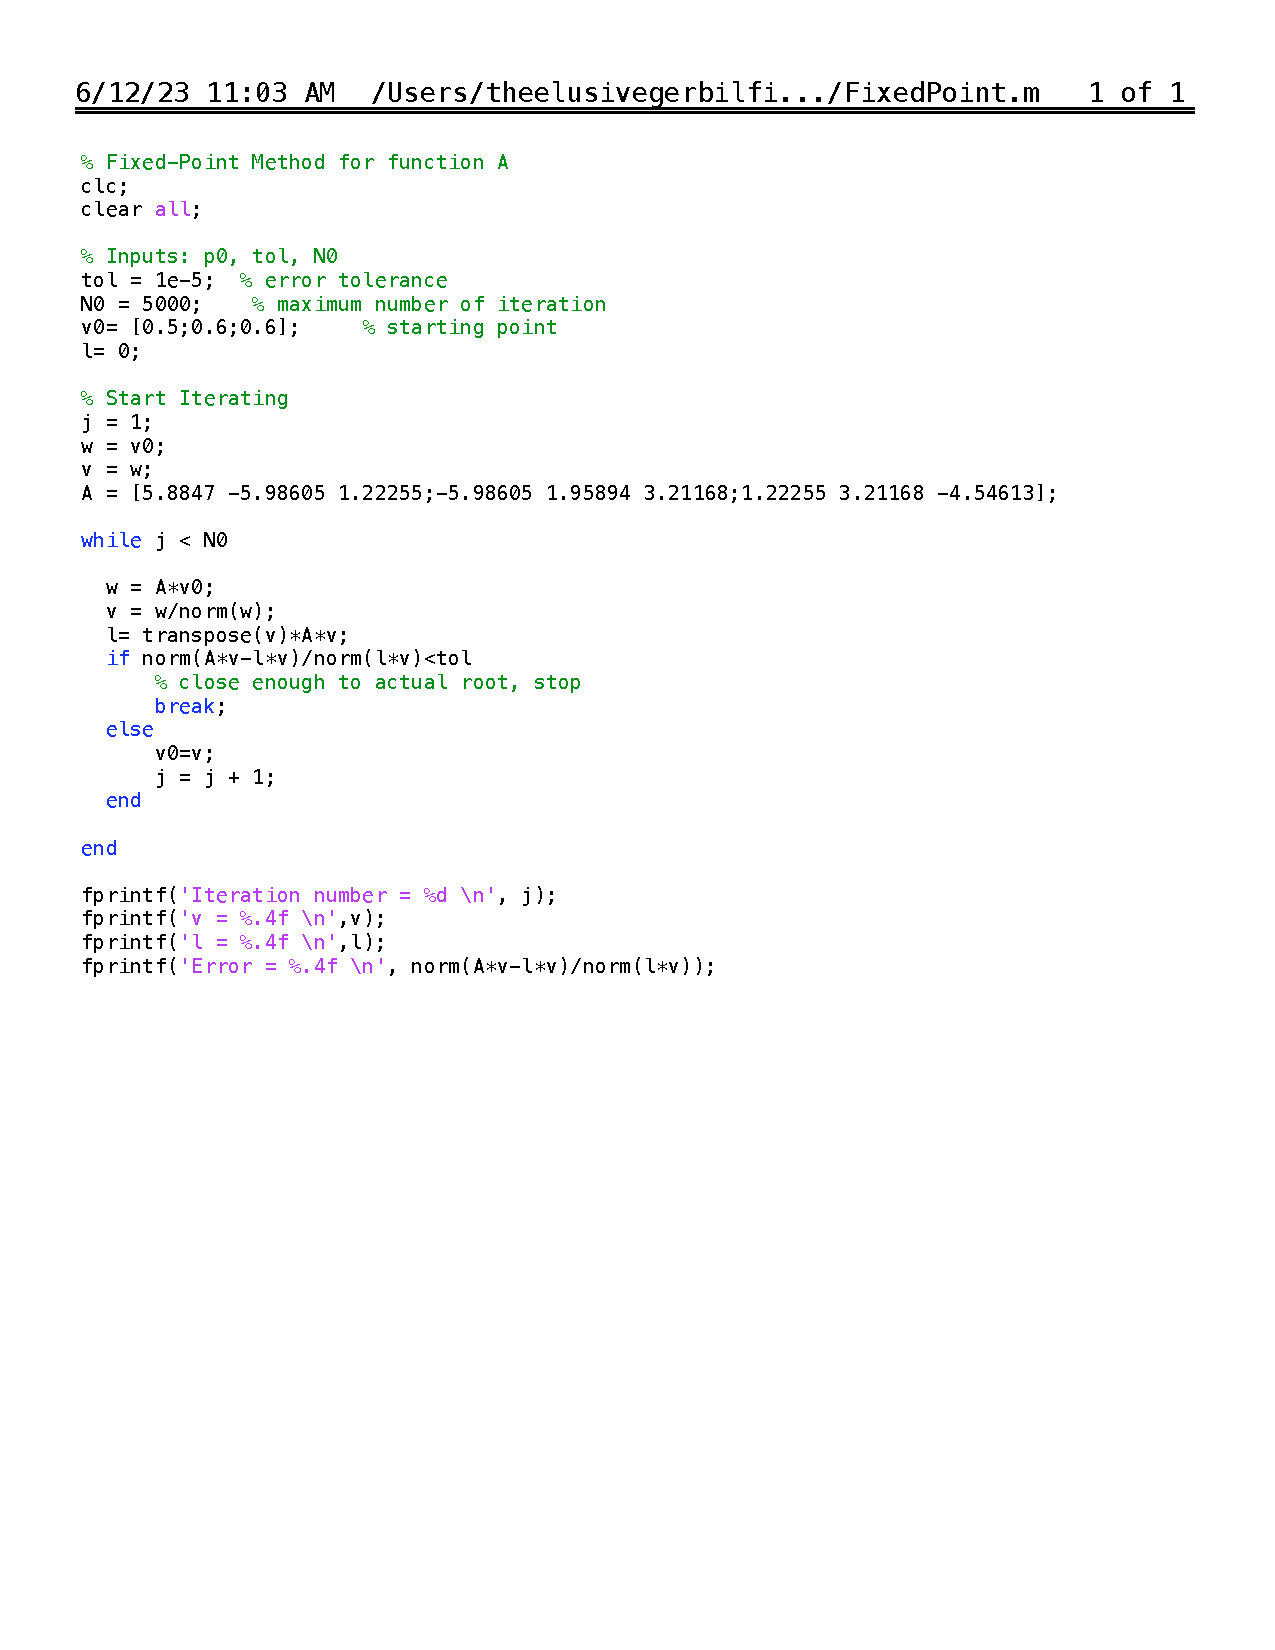
\includegraphics[width=\linewidth]{Fixed_point_final.pdf}
            \end{subfigure}%
            \begin{subfigure}{.5\textwidth}
                \centering
              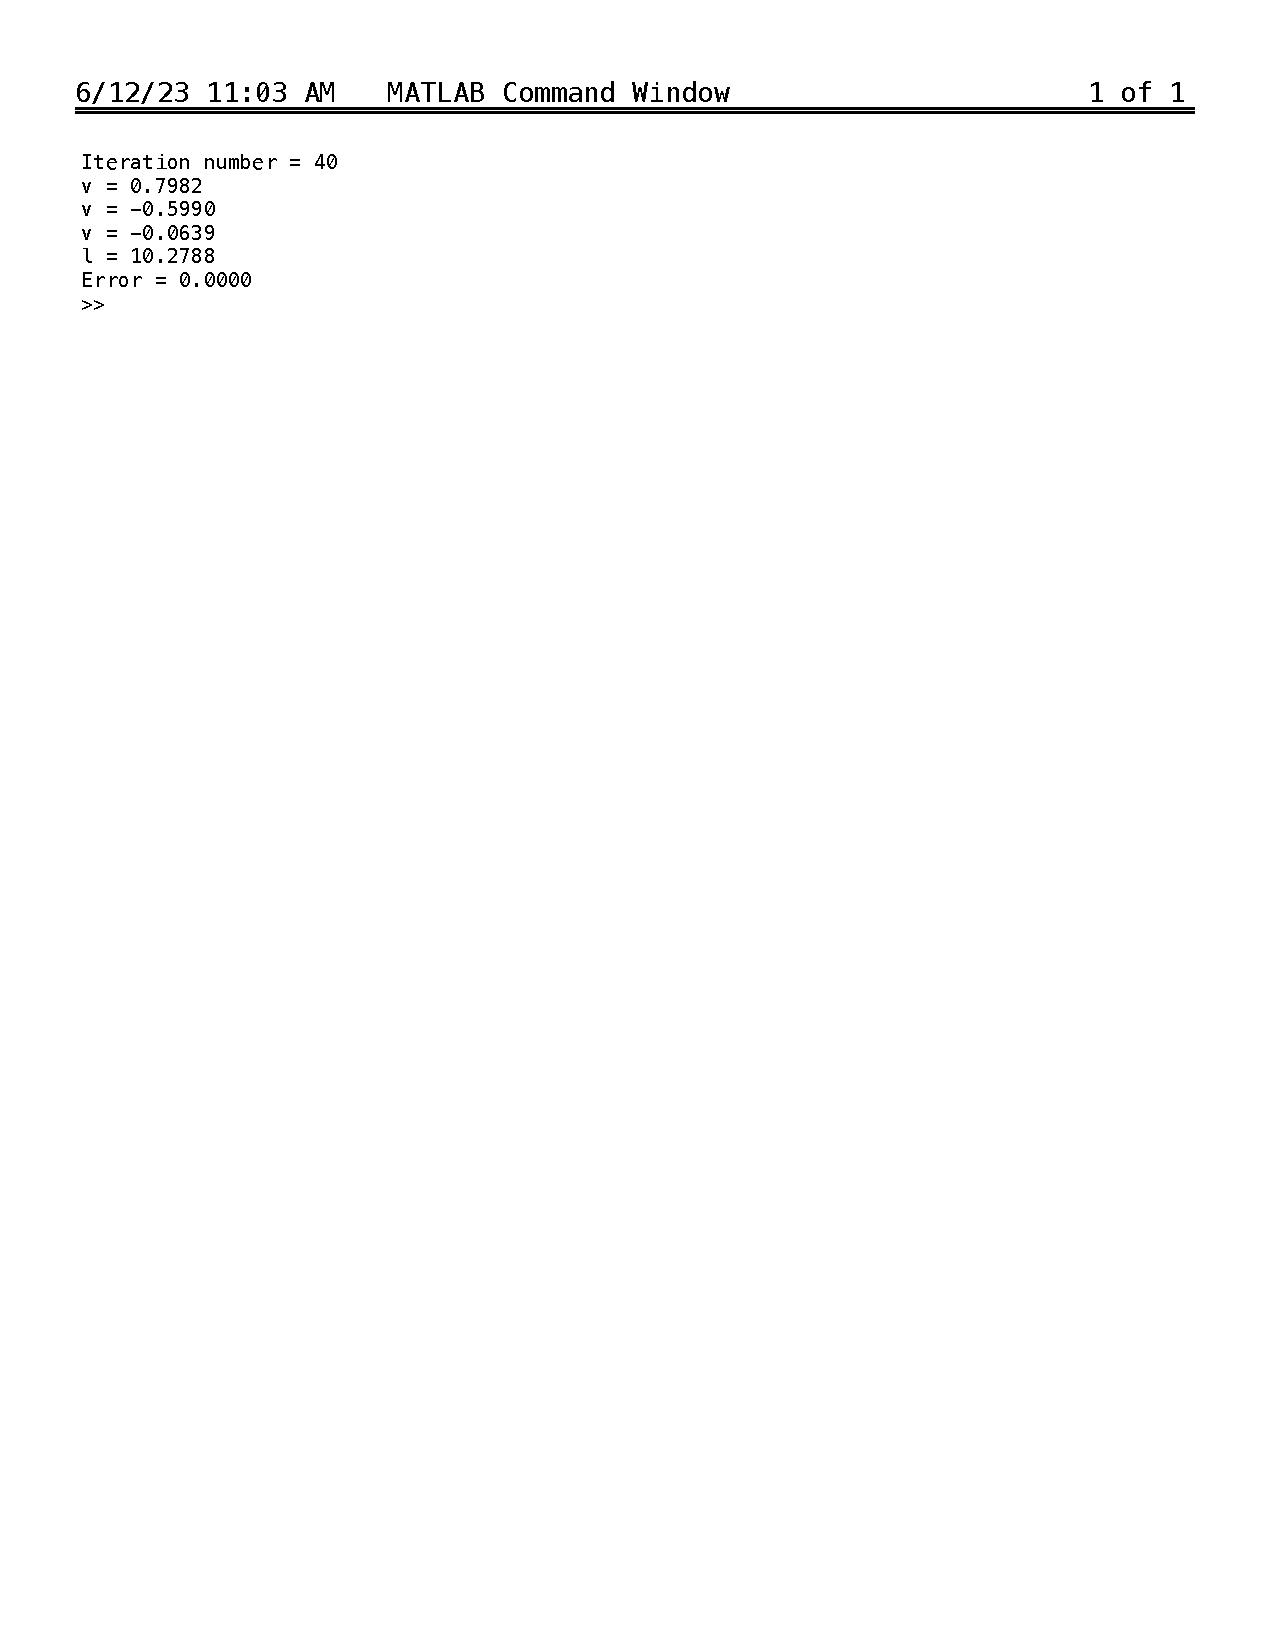
\includegraphics[width=\linewidth]{Fixed_point_command_window_final.pdf}
            \end{subfigure}
            \end{figure}
    \end{itemize}

\end{enumerate}

\end{document}